\documentclass{sig-alternate}[10pt]

% graphic declaration
\usepackage{graphicx}
\usepackage{listings}
\usepackage[english]{babel}
\usepackage{float}
\usepackage{color}
\usepackage{caption}
\usepackage{indentfirst}
\usepackage{amsmath}
\usepackage{fancybox}
\usepackage{algorithm}
\usepackage{algpseudocode}
\usepackage{multicol}
\usepackage{balance}
%\usepackage{svg}
\usepackage{pdfpages}

\definecolor{dkgreen}{rgb}{0,0.6,0}
\definecolor{gray}{rgb}{0.5,0.5,0.5}
\definecolor{mauve}{rgb}{0.58,0,0.82}

%\iffalse
%\lstset{frame=tb,
  %language=Java,
  %aboveskip=3mm,
  %belowskip=3mm,
  %showstringspaces=false,
  %columns=flexible,
  %basicstyle={\footnotesize\ttfamily},
  %numbers=none,
  %numberstyle=\tiny\color{gray},
  %keywordstyle=\color{blue},
  %commentstyle=\color{dkgreen},
  %stringstyle=\color{mauve},
  %breaklines=true,
  %breakatwhitespace=true,
  %tabsize=3
%}
%\fi

\lstset{%
  xleftmargin=0pt,
  belowcaptionskip=\bigskipamount,
  captionpos=b,
  escapeinside={*'}{'*},
  language=Java,
  tabsize=2,
  emphstyle={\bf},
  commentstyle=\it,
  stringstyle=\mdseries\ttfamily,
  showspaces=false,
  keywordstyle=\bfseries,
  morekeywords={then,end,String, Class, Object},
  columns=flexible,
  basicstyle=\scriptsize\ttfamily,
  showstringspaces=false,
  morecomment=[l]\%,
}

\graphicspath{ {data/} }

\begin{document}

\setcopyright{acmcopyright}
\conferenceinfo{MOBILESoft '16}{May 16--17, 2016, Austin, TX, USA}
\acmPrice{\$15.00}
%\doi{}

%
% paper title
% Titles are generally capitalized except for words such as a, an, and, as,
% at, but, by, for, in, nor, of, on, or, the, to and up, which are usually
% not capitalized unless they are the first or last word of the title.
% Linebreaks \\ can be used within to get better formatting as desired.
% Do not put math or special symbols in the title.
%\title{Expanding Limited Mobile Resources for Performance, Energy-Efficiency, and Privacy}
%\title{Extending Resource-Constrained Mobile Devices for Performance, Energy-Efficiency, and Privacy}
\title{Utilizing Nearby Distributed Computing Resources in Heterogeneous Mobile Network}
%Resource-Constrained Mobile Devices}

%%%N-REX (Nearby-Remote Executor similar to T-Rex)

% author names and affiliations
% use a multiple column layout for up to three different
% affiliations
\numberofauthors{2}
\author{
\alignauthor Le Dinh Minh \\
\affaddr{Department of Computer Science} \\
\affaddr{Utah State University} \\
\email{minh.le@aggiemail.usu.edu}
\alignauthor Advisor: Young-Woo Kwon \\
\affaddr{Department of Computer Science} \\
\affaddr{Utah State University} \\
\email{young.kwon@usu.edu}
}

% make the title area
\maketitle

\section{Problem}
These days, mobile devices have been significantly developed with powerful hardware facilities equipped such as multicore CPUs, large and fast memory, fast network and high resolution displays. As a result, mobile applications deliver increasingly complex functionality from the recent past. Furthermore, rapid growth in application functionality requires ever greater hardware capability. Thus ensuring the quality of service in resources-limited execution environments remains a major challenge of mobile software development. To reduce execution time and save battery power, some functionality of mobile applications is often executed at a remote server. However, such an optimization mechanism (i.e., computational offloading) has only received much attention in the research literature due to difficult implementation, limited applicability, cost of the cloud, etc. 

\begin{CCSXML}
<ccs2012>
<concept>
<concept_id>10010520.10010521.10010537</concept_id>
<concept_desc>Computer systems organization~Distributed architectures</concept_desc>
<concept_significance>100</concept_significance>
</concept>
<concept>
<concept_id>10010520.10010521.10010537.10010540</concept_id>
<concept_desc>Computer systems organization~Peer-to-peer architectures</concept_desc>
<concept_significance>100</concept_significance>
</concept>
</ccs2012>
\end{CCSXML}

\ccsdesc[100]{Computer systems organization~Distributed architectures}
\ccsdesc[100]{Computer systems organization~Peer-to-peer architectures}
\terms{Design}

\printccsdesc
\keywords{Mobile Application, Remote Execution, Offloading, Peer to Peer, Runtime System}


\section{Related Works}

The work presented here is related to other complementary efforts that optimize mobile applications via remote executions including computation offloading and peer to peer networking.

Alljoyn \cite{alljoyn} is an open source framework that hides the complexity of network communications for application programmers. By providing interoperability between multiple platforms without any transport layers, Alljoyn makes the integration and initiation of network communication easy and simple. Prior to the the Wi-Fi Direct technology, peer to peer networks have demonstrated the initiative steps to establish the point-to-point collaborative WiFi networks \cite{m_p2p_tutor}. 

In addition to the WiFi-based peer to peer network, there had been several efforts to use other communication medium such as bluetooth to share media contents \cite{media_share}. Rio \cite{rio} bases on I/O files to share contents and resources among the applications in different devices without having to modify them. Their use cases addressed multi-system photography and gaming, singular SIM card for multi-devices, music and video sharing. GameOn \cite{gameon} utilizes WiFi P2P to establish non-Internet connection between gamers with a focus on closed range networks like in public transportation. The other content sharing systems include CAMEO \cite{cameo}, Spartacus \cite{spartacus} and GigaSight \cite{crowd-sourcing}, which distribute data in closed range networks. By utilizing the Doppler effect, Spartacus help initiate and interact with nearby devices through pointing gesture with accuracy up to 90\% within 3 meters.

Finally, our work shares objectives and techniques with the well-known computational offloading approaches \cite{maui,comet,mobile-cloud-middleware,fuzzy-engine}. These offloading mechanisms is a well-known mobile application optimization technique that makes it possible to execute the application's energy intensive functionality at a powerful cloud-based server, without draining the mobile device's battery. In this research, we have focused on generalizing these offloading mechanisms using two different distributed execution models---client/server and peer to peer communication models.

\section{Solution}

\begin{figure}
	\centering	
		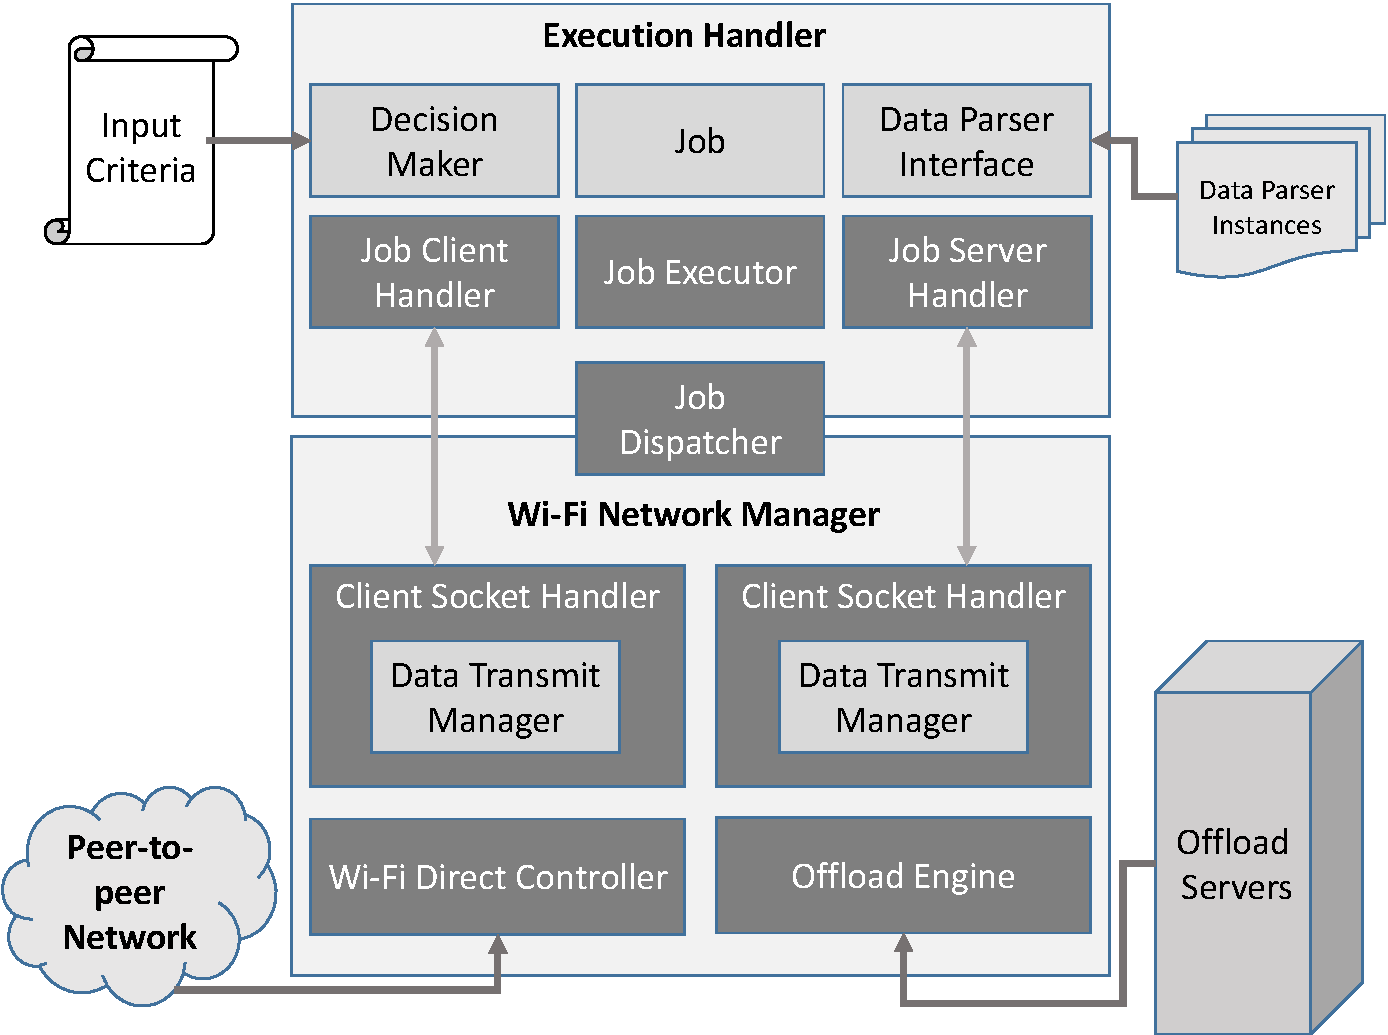
\includegraphics[width=.95\linewidth]{data/jobShareArch.pdf}	
	\caption{System architecture}
	\label{fig:architecture}
\end{figure}


\begin{figure} 
	\centering
	\resizebox{0.5\textwidth}{!}{
		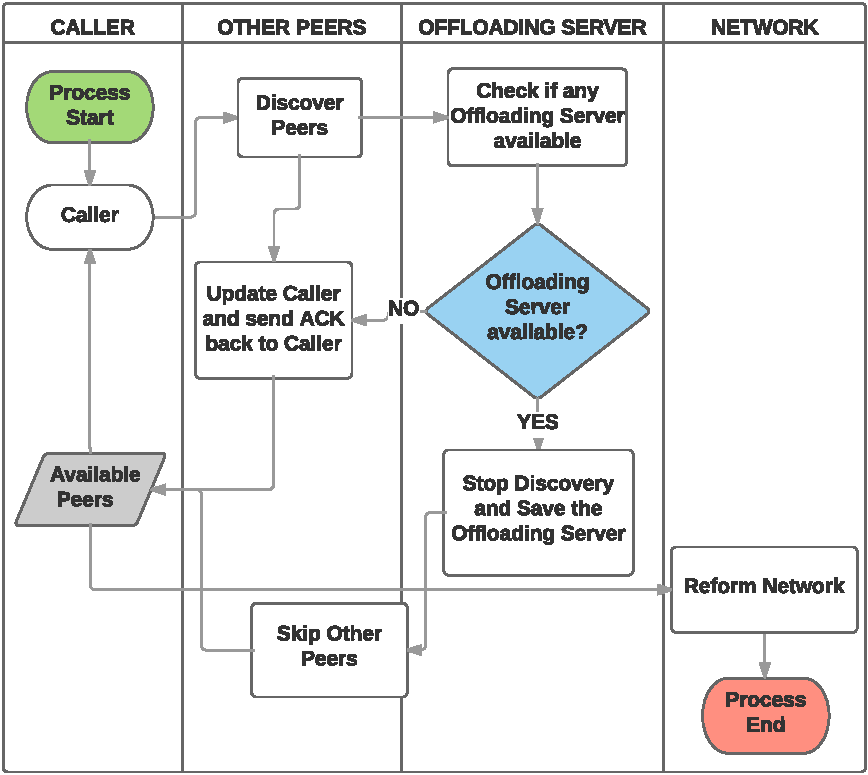
\includegraphics{data/discoverPeers.pdf}
	}
	\caption{Establishing a network connection between devices}
	\label{fig:forming}
\end{figure}

\subsection{Algorithms}

\subsubsection{Job quantitation for peers}\label{ss_jqfp}
To assign a job to multiple peers, the runtime system collects the available resource information from each mobile device. Specifically, the percentage of CPU usage is calculated using the \texttt{/proc/stat} system file as follows:
\begin{equation}
\label{eq:cpu_usage}
Usage_{CPU} = \frac{(\sum{T_{CPU2}} - T_{Idle2}) - (\sum{T_{CPU1}} - T_{Idle1})}{(\sum{T_{CPU2}} - \sum{T_{CPU1}})}
\end{equation}

\noindent where $\sum{T_{CPU}}$ is total active time and $T_{Idle}$ is idle time. For the memory usage, $Usage_{Mem}$ is calculated by accessing \texttt{MemoryInfo} of Android APIs such as $Mem_{Avail}$ and $Mem_{Total}$. Finally, we  calculate the battery usage, $Usage_{Batt}$. Next, to determine the appropriate amount of data to each mobile device, we introduce $RL$ parameter as follows:
\begin{equation}
\label{eq:res_level}
%\begin{\footnotesize}
RL = \frac{N_{Cores} \times CPU_{Speed}}{Usage_{CPU}} + \frac{Mem_{Spec}}{Usage_{Mem}} + \frac{Batt_{Spec}}{Usage_{Batt} \times 1000}
%\end{\footnotesize}
\end{equation}

\noindent where $RL$ is an indicator to the level of availability of mobile devices. The smaller $RL$ means the higher availability. $N_{Cores}$ is the number of CPU cores. $CPU_{Speed}$ is speed of single core in GHz. $Mem_{Spec}$ is the memory capacity in GB and $Batt_{Spec}$ is the battery capacity in uAh. For example, if $Usage_{CPU}$ is 0.3, $Usage_{Mem}$ is 0.5 (i.e., half of 1GB memory has been consumed), and $Usage_{Batt}$ is 0.7 or 70\% used over a 2800uAh capacity battery, then $RL$ will be $$RL = \frac{5.2}{0.3} + \frac{1}{0.5} + \frac{2800}{0.7 \times 1000} = 23.33$$

If the selected peer is a powerful cloud-based server, $Batt_{Spec}$ is considered $\infty$ and $Usage_{Batt}$ is 0. According to Equation \ref{eq:res_level}, $RL$ will also be $\infty$. To make the calculation simple, we assign the maximum value of Integer to $RL$. To reduce the calculation overhead on the calling side, $RL$ is prematurely calculated on each peer and then sent to the caller in response to the IRS request.

Finally, the \texttt{DecisionMaker} assigns the job with the appropriate amount of data ($M_{i}$) in accordance with the following equation:
\begin{equation} 
\label{eq:data_amount}
M_{i} = M\frac{RL_{i}}{\sum_{j = \overline{1,n}}{RL_{j}}}
\end{equation}

\noindent where $M$ is total size of data in bytes. $n$ is the number of mobile devices, where $i$-device has responsibility level $RL_{i}$. It is obvious that in the network with an offloading server, $M_{offload}$ is almost equal to $M$, and thus we can flush the full task with heavy computation to the offloading server. Algorithm \ref{alg:assign_job} describes how \texttt{DecisionMaker} assign a job appropriately while considering the availability of each mobile device. The algorithm returns the amount of data in binary length with two offsets that indicate the location of the data.


\begin{algorithm}

\caption{Selecting available peers}
\label{alg:select_peers}
\begin{algorithmic}[1] 
\begin{scriptsize}
\Function{selectPeers()}{}
\State Send IRS requests to all peers 
\State $CriteriaList \leftarrow IRSCriteria$
\State $P_{AV} \leftarrow HashMap(DeviceId, P)$

\If {$CriteriaList.RL = max$}
  \ForAll{$Resp_{IRS}$ in \{Incoming IRS Responses\}}
  	\State Find max $RL$ with other criteria in $CriteriaList$
		\State Assign device with max $RL$ to $P_{AV}$
  	\State \Return $P_{AV}$
  \EndFor
\EndIf

\ForAll{$Resp_{IRS}$ in \{Incoming IRS Responses\}}
  \If {$Resp_{IRS}[device] = server$}
  	\State Reset $P_{AV}$ 
  	\State $P_{Info} \leftarrow WiFiDevices.get(DeviceId)$
  	\State $P_{AV}[DeviceId] \leftarrow P_{Info}$
  	\State \Return $P_{AV}$
  \EndIf

  \If {All condition statements are satisfied} 
  	\State $P_{Info} \leftarrow WiFiDevices.get(DeviceId) + $
		\State
			\hspace{\algorithmicindent}
			\hspace{\algorithmicindent}
			\hspace{\algorithmicindent}
			\hspace{\algorithmicindent}
			$Resp_{IRS}[RL]$
  	\State $P_{AV}[DeviceId] \leftarrow P_{Info}$
  \EndIf
\EndFor

\State \Return $P_{AV}$
\EndFunction
\end{scriptsize}
\end{algorithmic}

\end{algorithm}


\begin{algorithm}
\caption{Assigning a job}
\label{alg:assign_job}
\begin{algorithmic}[1]
\begin{scriptsize}
\Function{assignJobs()}{}
\State $M \leftarrow {getDataSize()}$
\State $RL_{Total} \leftarrow 0$ 
\For {$P$ in \{$P_{AV}$\}}
  \State $RL_{Total} \leftarrow RL_{Total} + P[RL]$
\EndFor
\\
\State $firstOffset, lastOffset \leftarrow 0$
\State $jobData \leftarrow Null$
\State $job \leftarrow {readJobFile()}$
\State $M_{C} \leftarrow 0$
\\
\For {$i = 1$ to $P_{AV}.length$}\\
  \State $M_{i} \leftarrow M\frac{RL_{i}}{RL_{Total}}$\\
  \State $firstOffset \leftarrow M_{C} $
  \State $lastOffset \leftarrow M_{C} + M_{i}$
  \State $jobData \leftarrow DataParser.getSinglePart($
  \State 
		\hspace{\algorithmicindent}
		\hspace{\algorithmicindent}
		\hspace{\algorithmicindent}
		\hspace{\algorithmicindent}
		\hspace{\algorithmicindent}
						$firstOffset, lastOffset)$
  \State $dispatchJob(\{job, jobData\})$\\
  \State $M_{C} \leftarrow lastOffset$
  
\EndFor

\EndFunction
\end{scriptsize}
\end{algorithmic}
\end{algorithm}

\section{Technical Background}
In this section, we present the major technologies we used in this paper. The major technologies used in this work including computation offloading, remote execution, middleware, and WiFi direct. We will describe them in the following sub sections.

\subsection{Computational Offloading}   
Computation offloading has become a popular optimization technique for mobile applications \cite{maui,chun+:eurosys11,kwon+:icsm13,wen2012energy}. It leverages the resources of cloud-based remote servers to execute portions of a mobile application's functionality. By executing some of the application's functionality in the cloud, offloading reduces the amount of energy consumed by the mobile device, thus saving its battery power. An additional benefit of computation offloading is improved performance efficiency, as cloud servers have hardware resource more powerful that those available on mobile devices. This technique is used as one of the distributed execution model in this paper.

\subsection{Remote Execution and Middleware}
Our approach uses features from mainstream middleware mechanisms for distributed execution as building blocks. Middleware systems provide programming and runtime support to coordinates the execution of multiple remote processes. By eliminating the need for low-level network programming (e.g., managing sockets, marshaling/unmarshaling data, keeping track of processes), middleware offers convenient building blocks for constructing distributed systems. In our prior work \cite{kwon+:mobilesoft2015}, we introduced a programming model and a middleware architecture for performance and energy optimization. The runtime system developed in this paper is derived from our prior middleware design.

\subsection{WiFi Direct}
The WiFi Direct \cite{alliance2010wi} is a new peer to peer standard built on top of the IEEE 802.11 to provide direct connections between WiFi devices without an Internet connection. Over a WiFi network, a WiFi device can discover and connect to any types of WiFi devices without special configurations or setups. Once a connection is established, WiFi devices can communicate with each other as a client or an access point. WiFi Direct has been widely used to transfer content or share applications between mobile devices. Recently in Android, WiFi Direct has been available from Android 4.0 APIs. In this paper, our approach uses Android WiFi Direct \cite{wifi:p2p} to utilize nearby computing resources without an Internet connection or wireless access point (AP). Even though the discovery operation of WiFi Direct is costly \cite{trifunovic2013slicing}, our approach is still efficient for CPU-intensive executions and sharing hardware resources. 


\section{Contributions}
In this paper, we present a novel distributed execution model that not only optimizes mobile application's executions in terms of performance and energy efficiency, but also extends mobile device's hardware capability. In other words, mobile devices will be able to virtually add more hardware resources including computation, networking, memory, and sensors to the existing hardware setups. Our approach is realized as the following major technical solutions: (1) a straight programming model that enables the programmer to write any execution task and (2) a runtime system that determines an execution strategy and distributes the requested execution task over the nearby or remote network. Our runtime system employs a dynamic, adaptive mechanism to determine the best distribution and execution strategy under different execution environments including diverse network conditions and heterogeneous mobile devices.

The experiments in 3 case studies have demonstrated the effectiveness of our approach, to extend limited mobile hardware resources, thereby improving performance and energy efficiency as well as bringing new hardware capabilities. By presenting our approach, this paper makes the following technical contributions:
\begin{itemize}
	\item \textbf{Simple programming model:} We provide simple APIs for programmers to easily deploy distributed mobile applications to take full advantage of external remote resources using our distributed execution model.
	\item \textbf{Lightweight runtime system:} Our runtime system efficiently distributes executions to available peers or offloading server, based on a peer selection algorithm. 	
	\item \textbf{A proof of concept infrastructure implementation:} Through three case studies, our system demonstrates how mobile hardware resources can be effectively shared.
\end{itemize}

\section{Evaluation and Validation}
As compared to estimating the energy consumption in cellular networks, in a WiFi network the energy consumption can be easily estimated. The total energy consumption can be calculated as follows:
$$E_{0} = E + E_{w}$$
\noindent where $E_{w}$ is the energy that the app requires for waiting. Then, we calculate the energy consumed by sending a job to other peers through the WiFi Direct technology as follows:
$$E_{p2p} = E(\frac{RL_{0}}{\sum_{i = 1}^{n}{RL_{i}}}) + E_{WiFi} + E_{w}$$ 
\noindent $n$ is the number of devices. $RL_{i} (i = \overline{1,n})$ is the responsibility level of each mobile device. 

However, we do not consider $E_{w}$ because it will depend on the appearance of applications. For example, if an application has no GUI, $E_{w}$ will cause very little effect. From the two above equations, we can calculate the energy consumption differences between two job processing mechanisms:
$$E_{Diff} = E_{0} - E_{p2p}$$ 
or 
\begin{equation}
\label{eq:energy_diff}
E_{Diff} = E(1 - \frac{RL_{0}}{\sum_{i=1}^{n}{RL_{i}}}) - E_{WiFi}
\end{equation}

Since WiFi is known to drain a battery linearly by time during transmission \cite{wifi_energy}, particularly it can be represented by $y = 17.01x - 0.93$ for downloading and $y = 17.31x - 2.28$ for uploading, where $y$ stands for percentage of battery consumed when using Wi-Fi for a period of $x$ hours. Therefore, under non-adventitious circumstances, equation (\ref{eq:energy_diff}) infers that in a mobile system with a certain number of devices in different levels of responsibility, if E is big enough, or in other words, if the task to perform is big enough, then $E_{Diff} > 0$ will result in, thus deploying a peer-to-peer group will give a great benefit in terms of energy efficiency. The bigger value of $E_{Diff}$, the more benefit we will gain. 

In addition, if a cloud-based offloading server is available in the network, $RL$ and $E_{Diff}$ are calculated as follows: $\sum_{i=1}^{n}{RL_{i}} \rightarrow \infty$, $E_{Diff} = E - E_{WiFi}$ which is the maximum value under the same conditions.

\subsection{Case Studies}
To measure the performance of the system equipped with our APIs, we decorated a small testbed with collaboration of 5 different Android devices to perform our 3 test cases:
\begin{itemize}
	\item \textbf{Image Processing:} In this case study, we initiated a P2P network to blur a large size image, which could not be loaded and processed on a any single mobile device due to the limited memory space in mobile devices. Then, we distributed the blurring job to 1 to 4 mobile devices. 

\begin{figure*}
	\centering
	%\resizebox{0.39\textwidth}{!}{
	%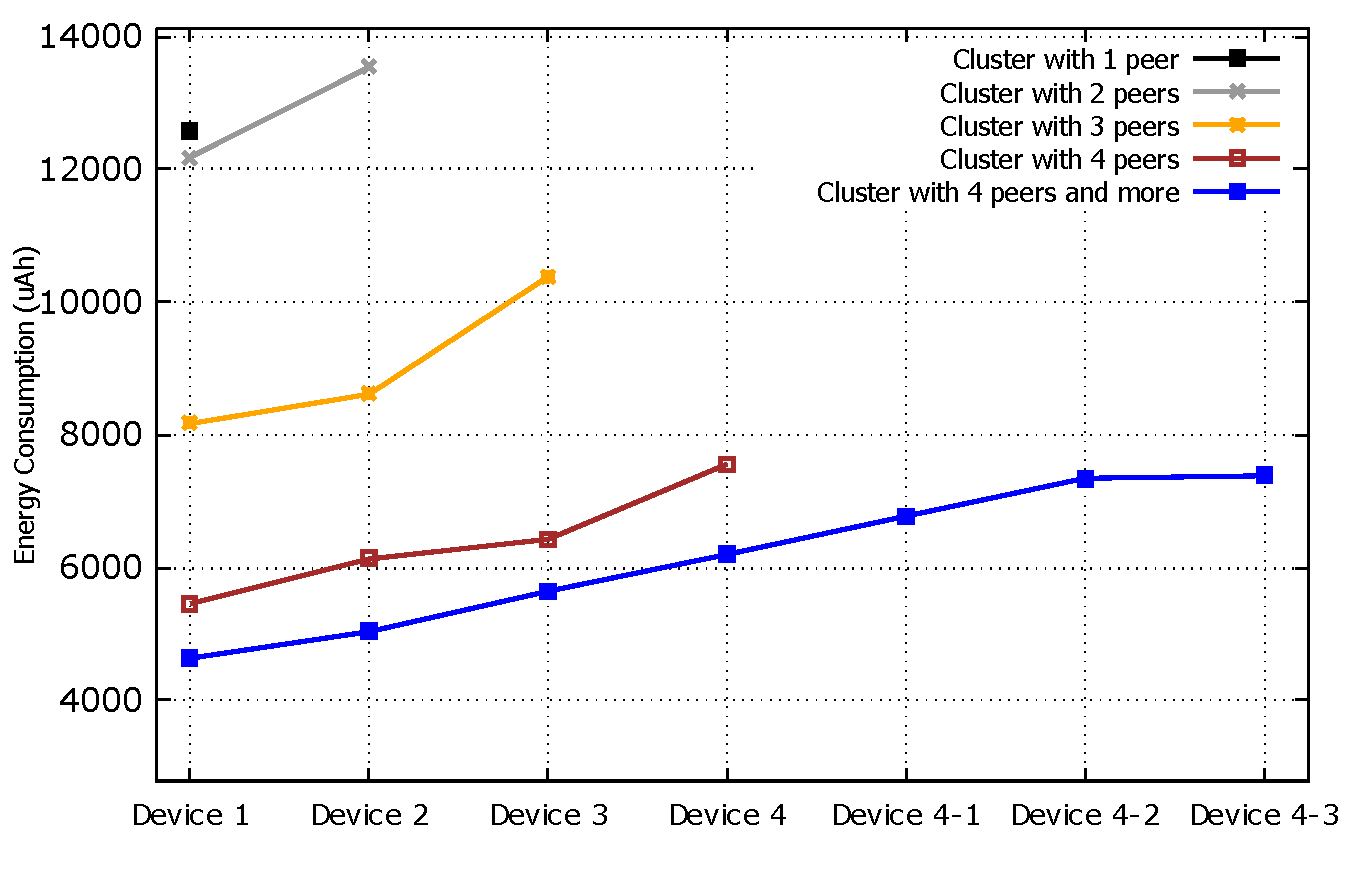
\includegraphics[width=0.32\textwidth]{data/img_large_perf_full.pdf}
		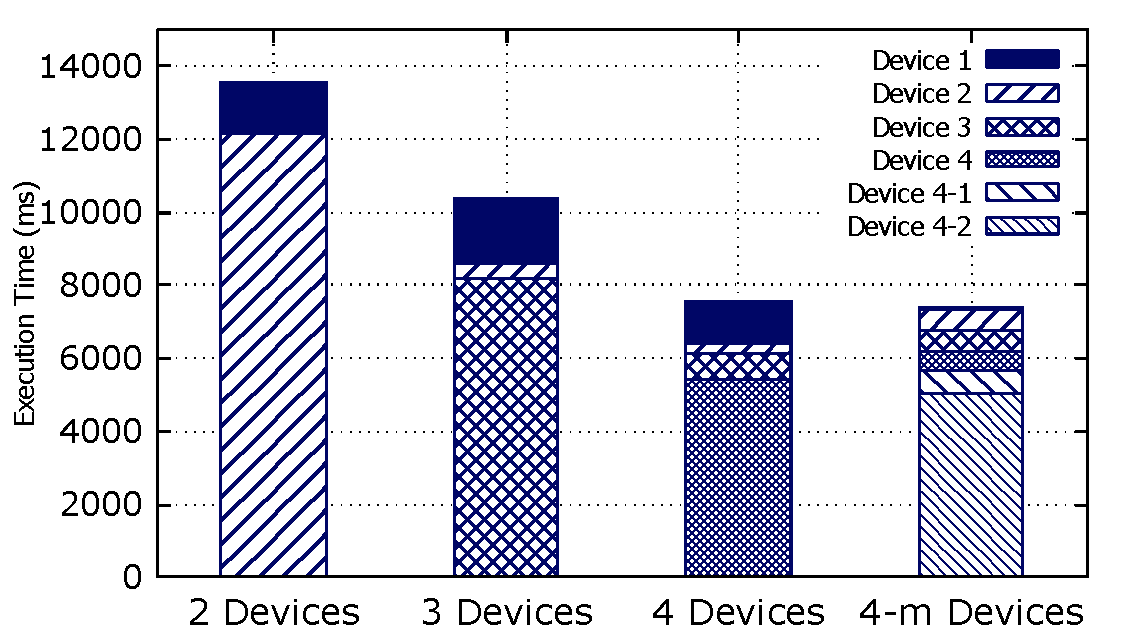
\includegraphics[width=0.43\textwidth]{data/img_perf.pdf}
		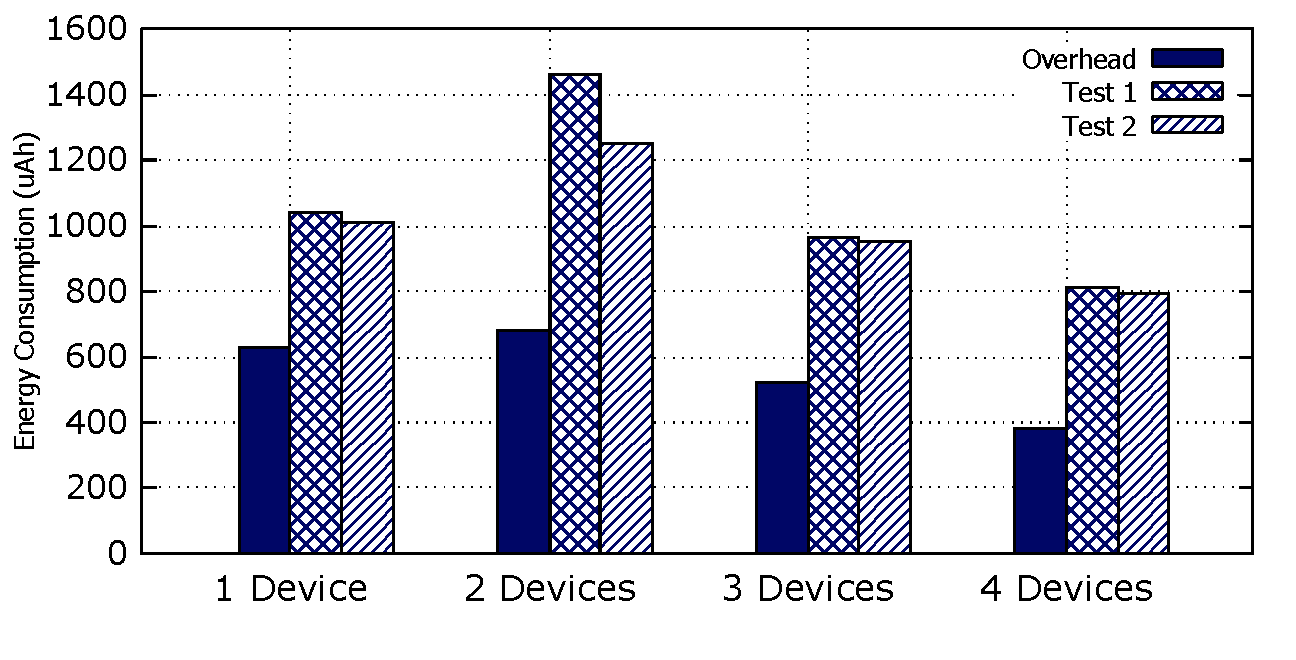
\includegraphics[width=0.48\textwidth]{data/img_energy.pdf}
	%}
	\caption{Performance and energy consumption of the large image processing tests in multiple devices.}
	\label{fig:cluster_performance}
\end{figure*}

\begin{figure*}
	\centering
	%\resizebox{0.45\textwidth}{!}{
		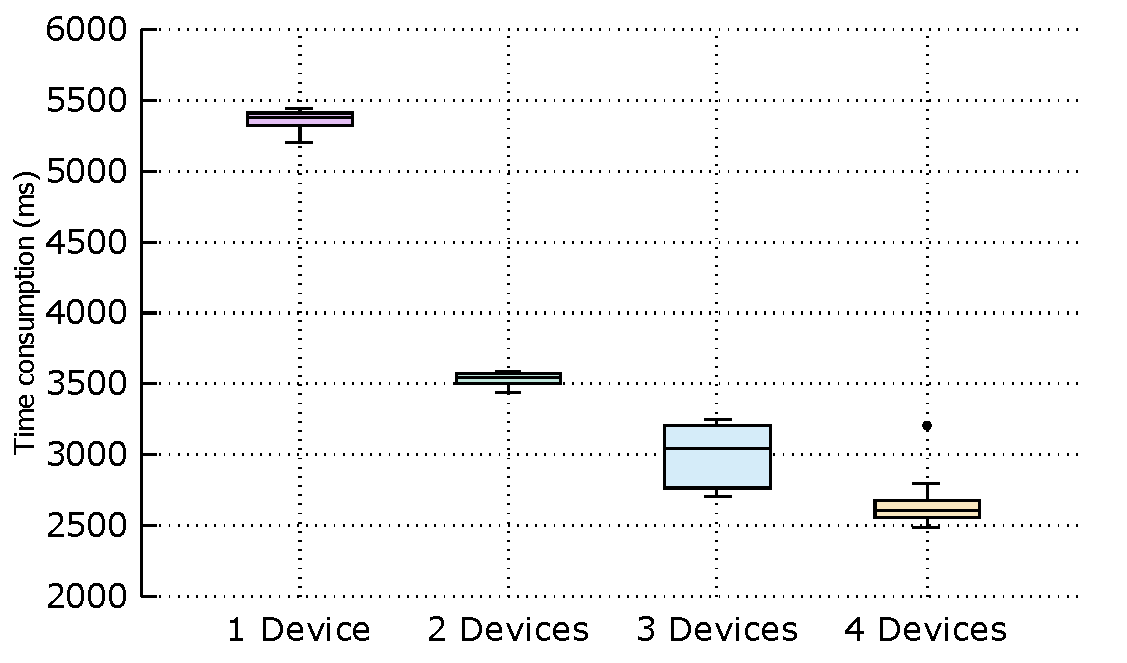
\includegraphics[width=0.48\textwidth]{data/img_small_perf_full.pdf}
		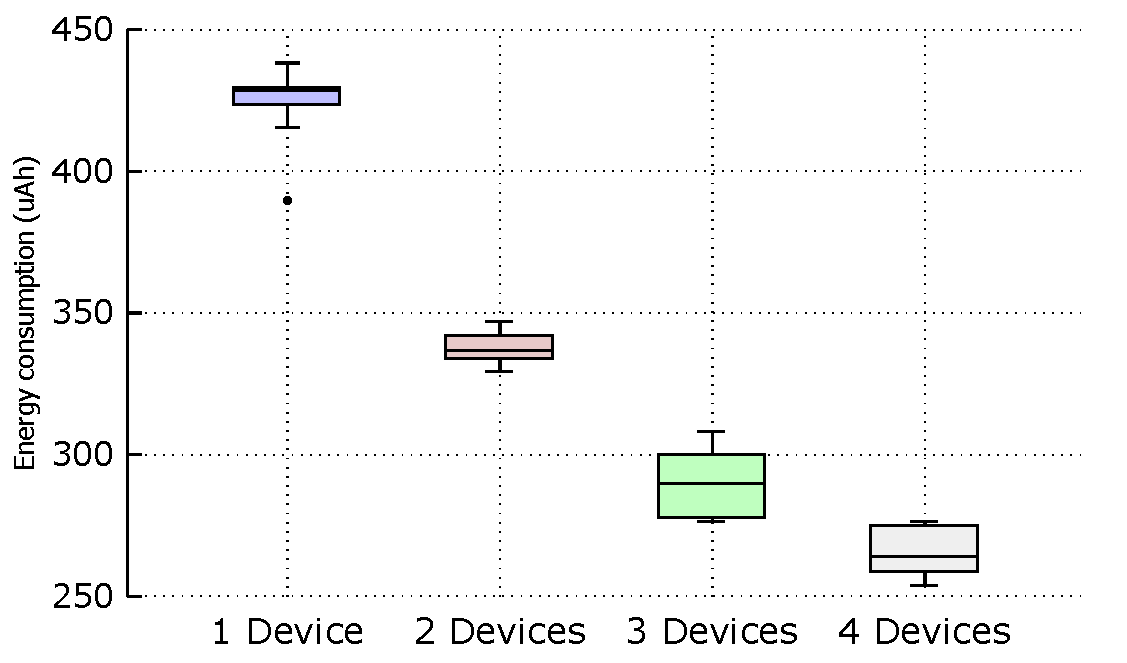
\includegraphics[width=0.45\textwidth]{data/img_small_energy.pdf}
	%}
	\caption{Performance and energy consumption of the image processing tests with a normal image size.}
	\label{fig:small_img_perf}
\end{figure*}


	
	%Particularly, to process an image with size $4000 \times 4000$ and 4 bytes to express each pixel color, application must spare the amount of memory equivalent to 64MB which is way too much for a device, which occasionally returns out of memory exception.
	\item \textbf{Internet Access:} In this scenario, we defined an Internet access request for a mobile device that has limited network connection or no Internet connection, so that mobile applications could download remote data.
	
\begin{figure*}
	\centering
	%\resizebox{0.45\textwidth}{!}{
		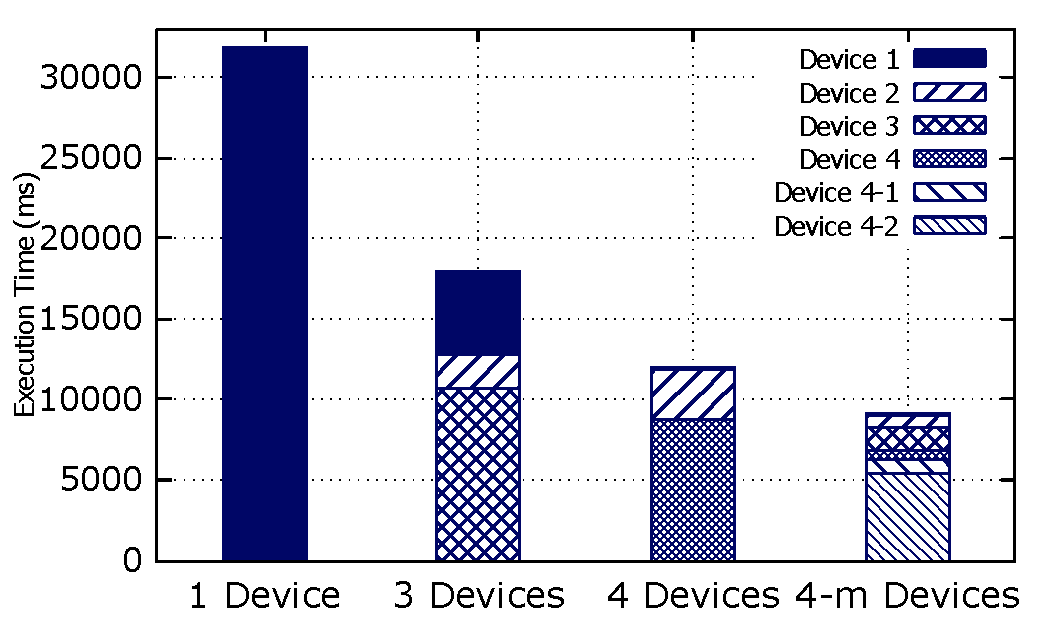
\includegraphics[width=.45\textwidth]{data/net_perf_01.pdf}
		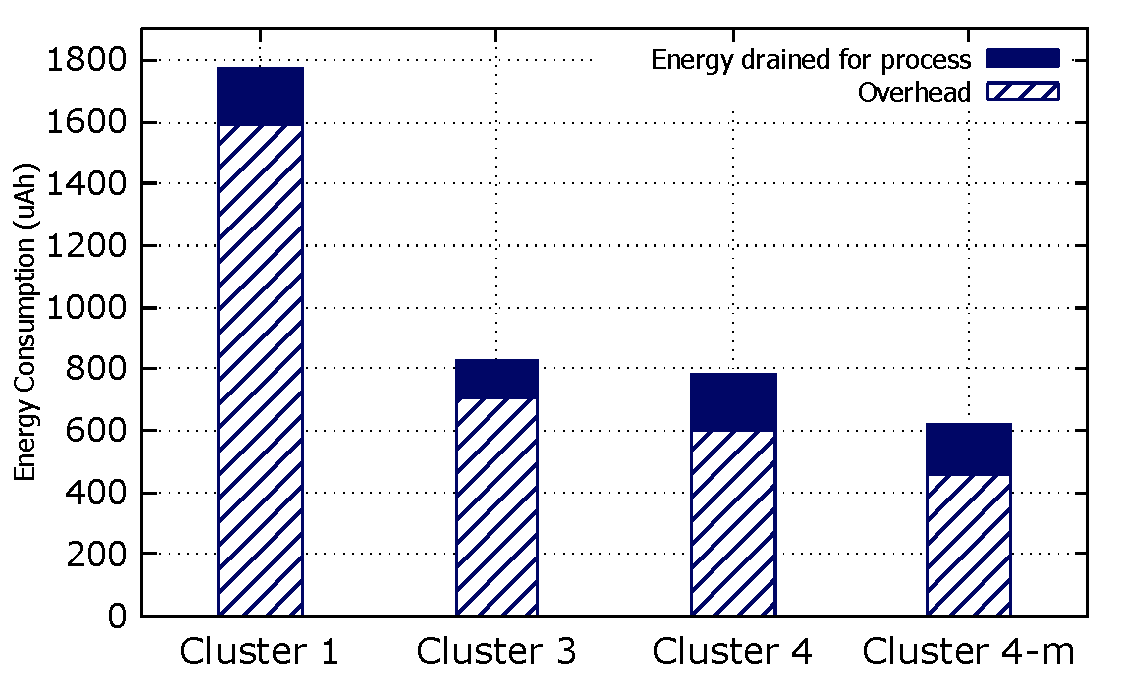
\includegraphics[width=.45\textwidth]{data/net_energy.pdf}
	%}
	\caption{Performance and energy consumption comparison for Internet sharing}
	\label{fig:net_clusters_perf}
\end{figure*}

	
	
	\item \textbf{GPS Sharing:} Because establishing a GPS connection is a highly energy-intensive operation, it would be impossible for a device with low battery to frequently update its location information. We built a simple application that can benefit GPS locations from healthier devices. In addition, our system can be used for Internet of Things devices that do not have GPS sensors.
\end{itemize}
\begin{figure*}

	\centering
	%\resizebox{0.36\textwidth}{!}{
		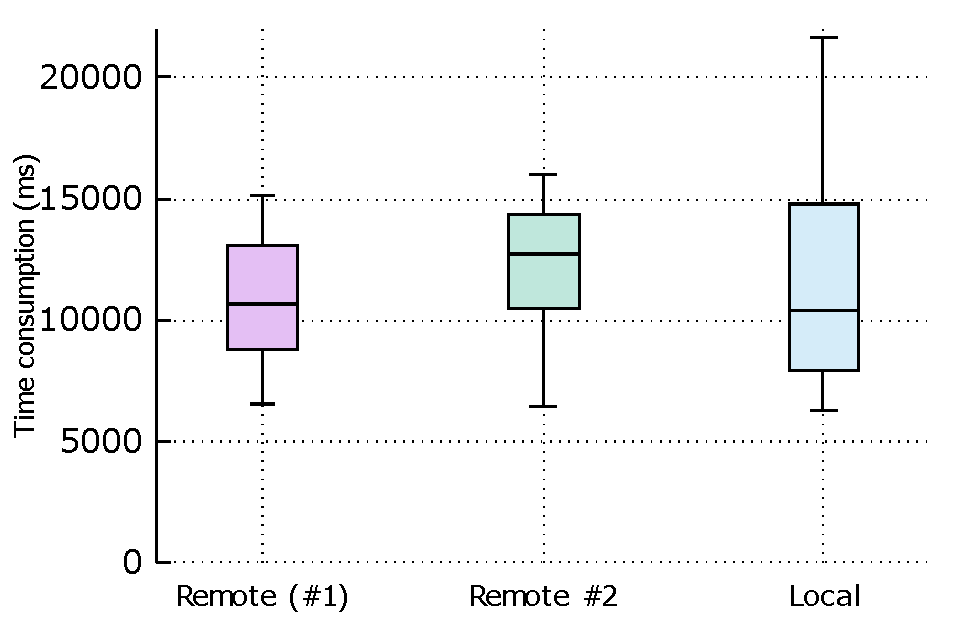
\includegraphics[width=.42\textwidth]{data/gps_perf.pdf}
		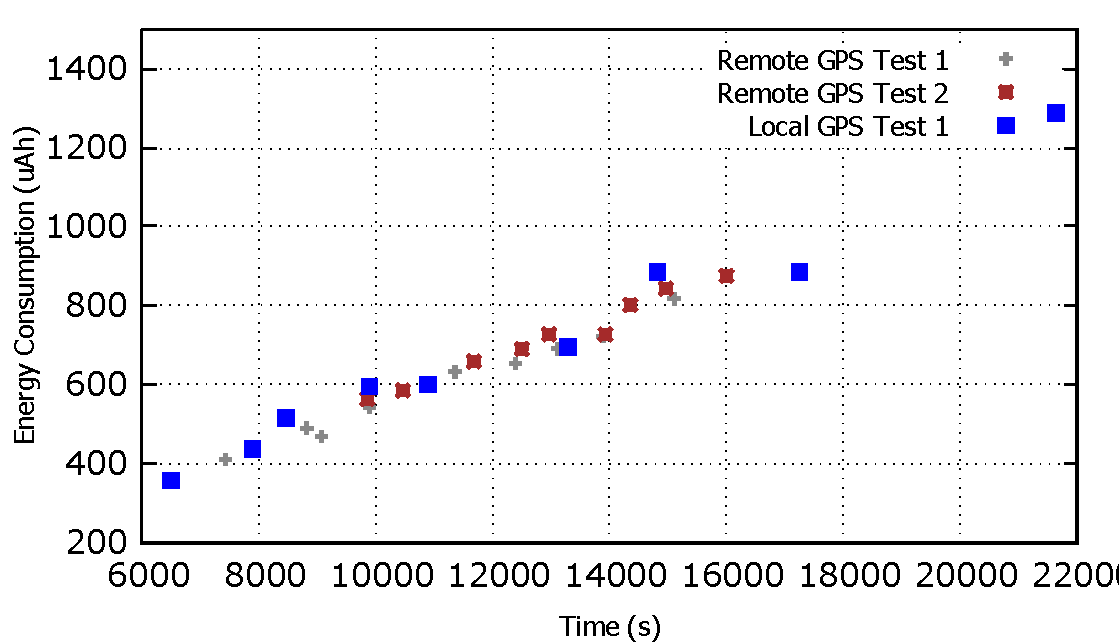
\includegraphics[width=.47\textwidth]{data/gps_energy_full.pdf}
	%}
	\caption{Performance and energy consumption comparison between remote and local GPS sensing.}
	\label{fig:gps_perf}
\end{figure*}


\section{Current Implementation}


In this paper, we present a novel distribution infrastructure that executes any functionality at a powerful remote server or nearby mobile devices using two distributed execution models---client/server and peer to peer. By means of a simple programming model, the programmer can easily adopt two distributed execution models in their applications. Our benchmarks and case studies demonstrate that the new distribution infrastructure can increase both performance and energy efficiency of mobile applications as well as introducing new feature (i.e., sensors) to the existing mobile devices.


\balance
\bibliographystyle{abbrv}
\bibliography{references}

\end{document}

